%released
\documentclass[../_main/handlingar.tex]{subfiles}

\begin{document}
\proposition{Renovering av Diplomat och allmäna utrymmen}

Hotell Diplomat är ett bra rum för att kolla på film i men är svårt att använda till mer än det. Styrelsen ser en stor potential i att använda rummet mer om man ersätter den blå soffan med mindre enskilda soffor som både kan möbleras i samma formation som den nuvarande men även i mindre soffgrupper. Mindre soffgrupper hade givit större möjligheter att sitta och äta i grupper på lunchen samtidigt som det ger upphov till fler studiplatser i Edekvata.

\begin{center}
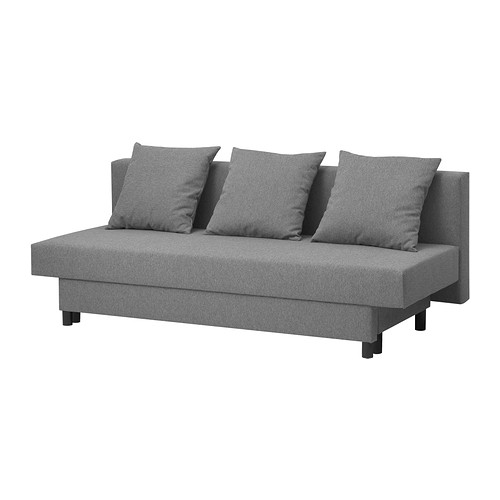
\includegraphics[width=7cm]{asarum.jpg}
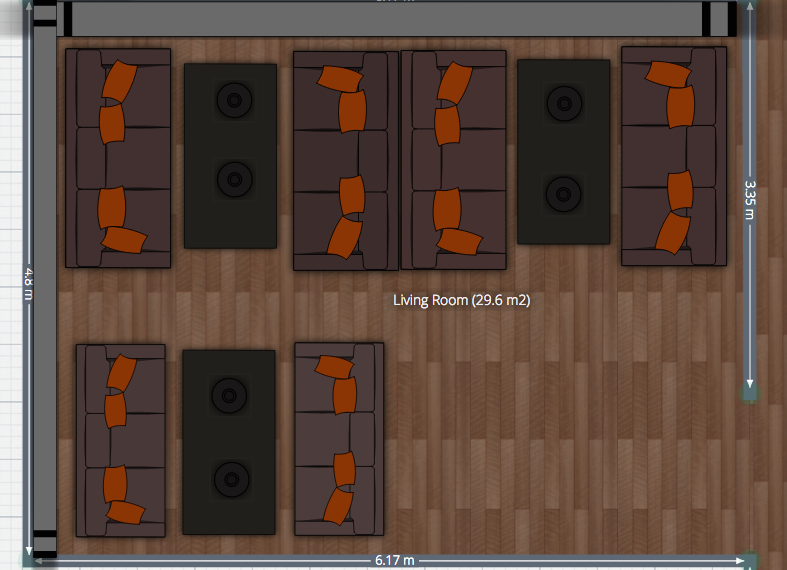
\includegraphics[width=7cm]{diplomat.png}
\end{center}

Därför yrkar vi på
\begin{attsatser}
    \att köpa in 6st mindre soffor, av modell ovan.
    \att köpa in yttligare belysning till Diplomat för att ge en bättre koncentrerad belysning över dem mindre soffgrupperna.
    \att en budget på 25000kr avsätts till projektet.
    \att kostnaden belastar utrustningsfonden.
\end{attsatser}

\begin{signatures}{2}
    \ist
    \signature{Anders Nilsson}{Förvaltningschef}
    \signature{\ordf}{Ordförande}
\end{signatures}

\end{document}
